\documentclass[12pt, a4paper]{article}
\usepackage[utf8]{inputenc}
\usepackage{amsmath}
\usepackage{hyperref}
\usepackage{enumitem, graphicx}
\usepackage{array}
\usepackage[margin=0.8in]{geometry}

\setlength{\parindent}{0pt}
\setlength{\parskip}{0.5em}

\makeatletter
\renewcommand{\@seccntformat}[1]{\csname the#1\endcsname.\quad}
\makeatother

\title{The Control System of the V-2}
\author{Otto Müller\footnote{Dr.-Ing. — Formerly: Stellvertrelender Abteilungsleiterr, Elektromechanische Werke, Karlshagen, Germany. — At present: "Attaché au service technique de l'armée française, Vernon, Eure, France.}}
\date{}

\begin{document}
\maketitle
\tableofcontents

\newpage
\section[The Control Problem and the Required Control Circuits]{The Control Problem and the Required Control\\Circuits}

The long range rocket V-2 was designed to transport its warhead to a target about 250 km away. It was to reach this target as an unpropelled projectile after the thrust had been cut off. Simple calculations showed that the maximum range for a given velocity at all-burnt was obtained with an angle of 49$^\circ$ between trajectory tangent and the vertical. Because of the starting weight of 12.5 tons, the normal type of inclined launching ramp would have been too heavy. Thus the rocket had to undergo a change of direction after launching; for this a control loop, the so-called pitch control, was required.

Furthermore, a control in yaw had to be incorporated, for without this the rocket would have deviated too much from its intended trajectory in the lateral direction.

A third control loop was required to suppress the natural tendency of the rocket to roll due to structural inaccuracies. It was not permissible to let the V-2 roll, because, as we shall see later, the control equipment contained gyros.

\begin{figure}[ht]
  \centering
  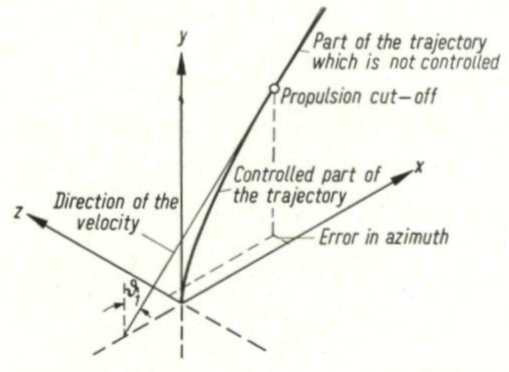
\includegraphics[width=0.6\textwidth]{figs/ctrl-01.png}
  \caption{The first part of the trajectory of the V-2.}
  \label{fig:01}
\end{figure}

In order to obtain the desired range, the thrust — after the end of the directional change — had to be cut off when the rocket had reached a predetermined velocity. For this purpose, a device had to be developed by which the velocity of the rocket could be measured and the fuel shut down, when the ``all-burnt-velocity" had been reached. Fig. \ref{fig:01} shows the first part of a trajectory of a V-2 rocket.

\section{The Control Equipment for the Standard Series}

\subsection{The Automatic Pilot for Yaw, Pitch, and Roll}

For the directional control of the rocket, the automatic pilot with gyros as used in aircraft readily suggested itself. We shall consider the control in yaw first. A potentiometer attached to a gyro produced a voltage proportional to the angle between the actual and intended direction of the axis. The voltage, via a stabilizing network and two amplifiers in parallel, operated a couple of servo units (Fig. \ref{fig:02}).

\begin{figure}[ht]
  \centering
  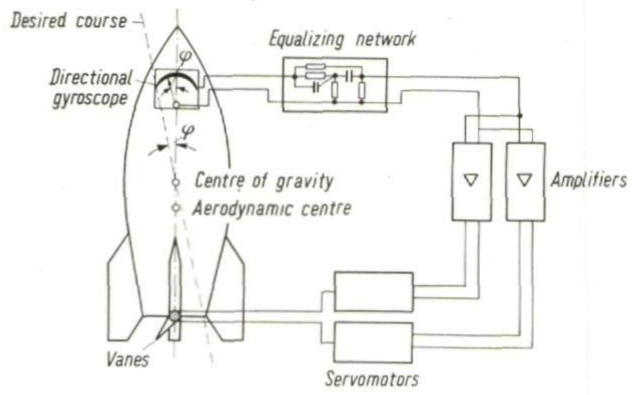
\includegraphics[width=0.7\textwidth]{figs/ctrl-02.png}
  \caption{Scheme of the control in yaw.}
  \label{fig:02}
\end{figure}

The particular difficulties in designing the control circuit were as follows:

\begin{enumerate}
  \item Only a velocity servo was available as a servo drive, since at that time it was used in aircraft.
  \item The aerodynamic forces varied considerably during flight. The velocity of the rocket and the density of the air varied by several orders of magnitude, and the distance between the centre of pressure and the centre of gravity by a factor of 10.
\end{enumerate}

However, a solution was found, in with a passive network was used and the amplification as well as the transfer function of amplifier and network were kept constant from start to all-burnt, this being extremely desirable for technical reasons. In order to avoid tedious repetition we shall consider at a later stage Low this solution was found.

The degree of feed-back was chosen so high that the control circuit was just sufficiently damped throughout the control time. This is not a priori the best solution: an accelerated unguided rocket veers into the wind, whereas a guided rocket with a high degree of feed-back in its controls drifts with the velocity component of the wind normal to the assigned trajectory. Therefore there is a certain degree of feed-back for which the wind has no influence on the lateral motion. Calculations, however, showed that for all disturbing forces occurring laterally, the accuracy in yaw was best in the case of highest possible degree of feed-back in the control circuit.

Graphite controllers were used as control vanes in the venturi with, for reasons to be explained later, small air-vanes in parallel. Controllers in the venturi were used for two reasons:

\begin{enumerate}
  \item The relatively long time during which the rocket had to travel, because of its small initial acceleration, in order to develop at the air-vanes reaction forces sufficient to counterbalance wind and thrust unsymmetries, would have been sufficient to make the rocket turn through 90$^\circ$.
  \item The available hydraulic servo units were of rather low performance. It was therefore necessary to use well balanced controllers, i. e. of a type with a very small torque. It was not thought possible that within permissible: time air-controllers could have been developed which, for the whole velocity range (MACH number 0 to 6), would be sufficiently balanced.
\end{enumerate}

After many trials, graphite controllers of such a shape were developed for use in the venturi that, in spite of loss through burning, equilibrium was sufficiently- retained for the whole of the trajectory. One may say that the low performance of the servo units prevented the development of a really good yaw control circuit for the V-2.

\begin{figure}[ht]
  \centering
  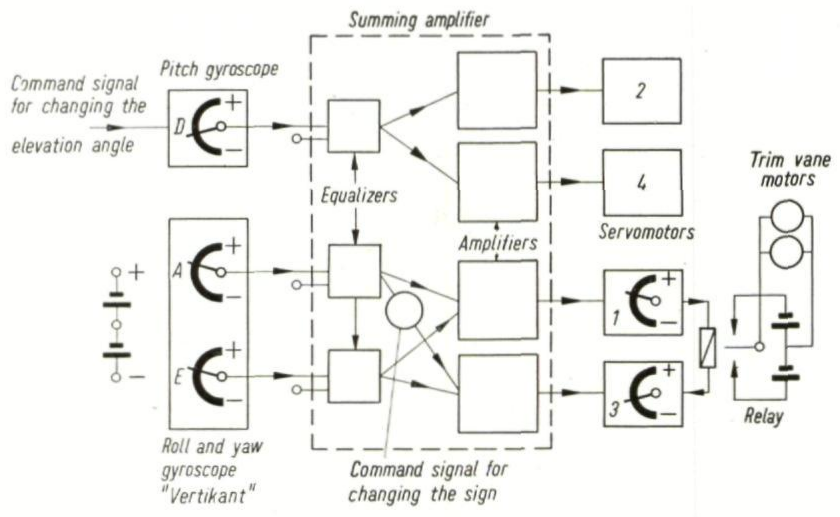
\includegraphics[width=0.75\textwidth]{figs/ctrl-03.png}
  \caption{Block diagram of control in yaw, pitch, and roll.}
  \label{fig:03}
\end{figure}

The control in pitch was nearly identical with the control in yaw. Only the direction assigned to the roll axis (direction of course) was varied in time so that the desired direction of the trajectory and thus the desired change in direction was obtained. The direction of the course and the trajectory tangent were nearly identical in the case of the V-2-control systems. For the chosen trajectory the angle of attack remained always smaller than 3$^\circ$, and the angle between the axis of the rocket and its assigned direction never exceeded the same value because of the high degree of feed-back in the control circuit. The accurate calculation of the assigned direction from the desired trajectory tangent is not difficult.

In the first controlled rockets the direction of the course was changed by making the gyro precess by a signal (the precession axis was called D-axis). The direction of the course was the direction of the spin axis of the gyro. Later on, the pick-off pitch was given as angular deviation with respect to the rocket; in this method, which yields better results, the direction of the course differs from the axis of the gyro by this angular deviation.

The control circuit for roll was identical with the control in yaw up to the amplifier input, only the network was somewhat different. The output voltage of the network was fed into both amplifiers for yaw control, from which one feed line passed through a phase-inverter. The roll signal thus operated the yaw controllers in phase opposition. We now understand the purpose of the small additional air controllers: because of their small leverage about the longitudinal axis the effectiveness of the controllers in the venturi was not sufficient to counterbalance the moments in roll. It was found that even the additional air controllers had insufficient effect. Therefore a so-called ``Trimmsegclsteuerung" was built into the tail plane which, by way of a control circuit making use of integrated deviation, compensated continuous disturbances in roll. Fig. 3 shows a circuit diagram of the direction and roll control circuit. We see that a gyro, a so-called ``Vertikant", carried the yaw and roll pick-offs; the amplifiers and networks were combined in the so-called mixer unit (summing amplifier)

\begin{figure}[ht]
  \centering
  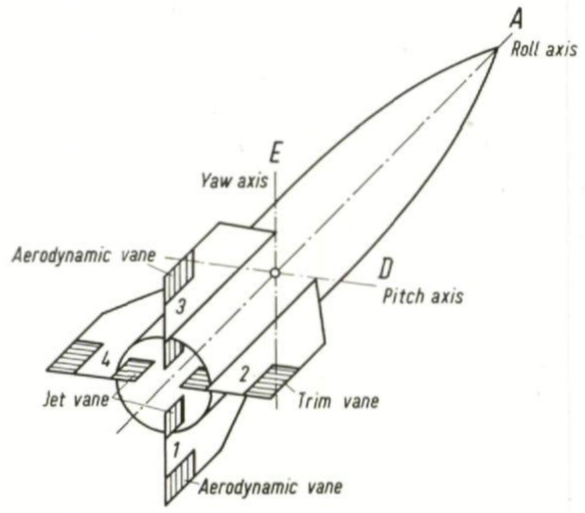
\includegraphics[width=0.6\textwidth]{figs/ctrl-04.png}
  \caption{Location of vanes of the V-2.}
  \label{fig:04}
\end{figure}

Fig. 4 shows the arrangement of the control vanes. The functioning of the trim vanes destabilizes the control in roll, but only to a permissible degree.

Special care has to be taken with regard to the correct position of the assigned course during launching and flight. In order to satisfy the first condition, the gyros were mounted on a kind of adjustable platform. The rocket was adjusted so that the platform was in a horizontal position, and one of its edges pointed towards the target (optical adjustment by collimator) (see Fig. \ref{fig:05}). To make sure of the second condition, gyros were used, which in the laboratory did not wander more than 0.1 to 0.2 degrees per minute under the influence of gravity.

\begin{figure}[ht]
  \centering
  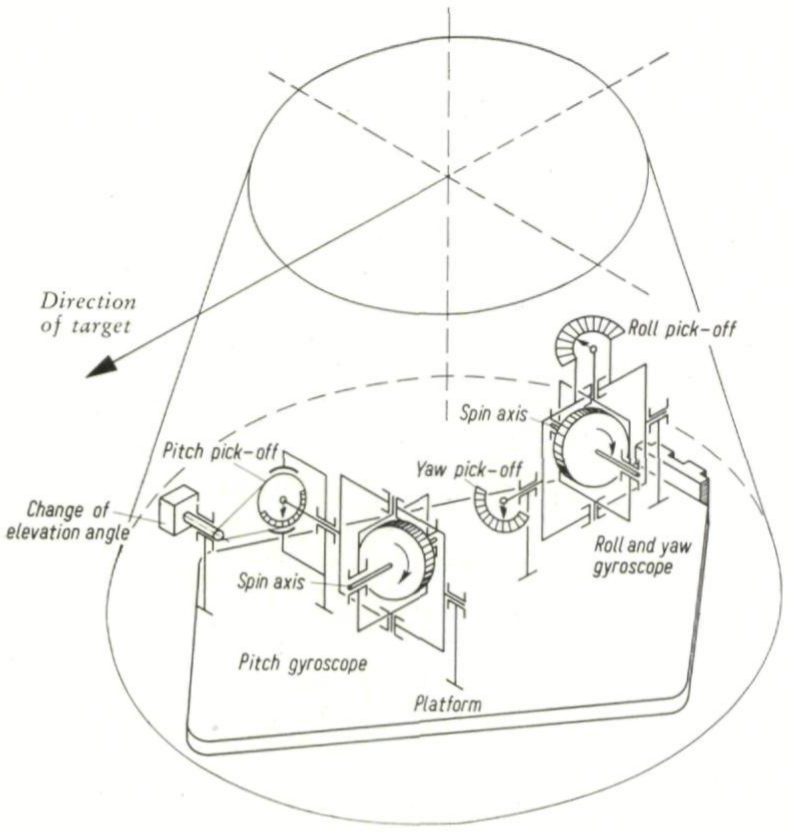
\includegraphics[width=0.7\textwidth]{figs/ctrl-05.png}
  \caption{Arrangement of the gyroscope in the missile.}
  \label{fig:05}
\end{figure}

\subsection{Fuel Control}

\subsubsection{General}

For the range of the rocket we have as first approximation

\begin{equation}
  X=f(v_{1})\quad\quad v_{1}=\text{ fuel cut-off or all-burnt velocity).}
\end{equation}

The fuel cut-off unit had to shut down the fuel supply when the rocket had reached the velocity assigned $v_{1}^{*}$. It consisted as is shown in Fig. \ref{fig:06} of,

\begin{enumerate}
  \item a device for measuring the rocket velocity, furnishing a quantity $B$ proportional to this velocity near the cut-off point;
  \item a device (comparator) releasing a signal when $B$ exceeded a predetermined
quantity $A$;
  \item a relay operated by this signal which shut down the supply of fuel to the
combustion chamber.
\end{enumerate}

\begin{figure}[ht]
  \centering
  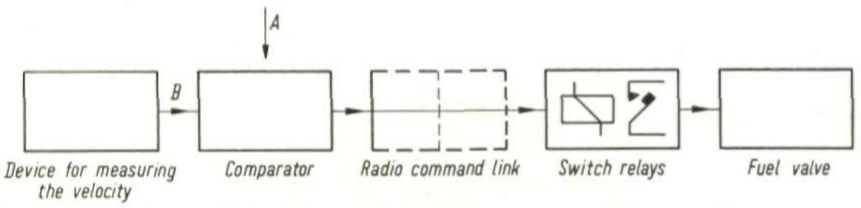
\includegraphics[width=0.8\textwidth]{figs/ctrl-06.png}
  \caption{Block diagram of the device for propulsion cut-off.}
  \label{fig:06}
\end{figure}

If the velocity measuring equipment was stationed on the ground an additional radio transmitter unit was required.

The quantity $A$ is approximately proportional to the all-burnt velocity $v_{1}^{*}$. However, since the rocket velocity still increases in the time between the response of the comparator and the complete cessation of combustion, $A$ was actually chosen to be proportional to a velocity which was smaller than the all-burnt velocity assigned by the mean value $\Delta v_{1}^{*}$ of this increase $\Delta v_{1} $. Since the variance of $\Delta v_{1}$ , was relatively large, $\Delta v_{1}$  was reduced by reducing the thrust immediately before cut-off in the ratio 4:1 . This produced a thrust-time curve as shown in Fig. \ref{fig:07}. Further corrections of $A$ will be discussed later-

\begin{figure}[ht]
  \centering
  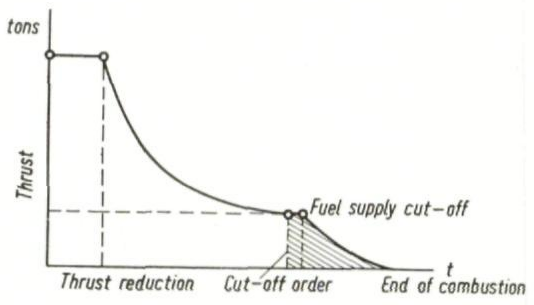
\includegraphics[width=0.6\textwidth]{figs/ctrl-07.png}
  \caption{Thrust at cut-off.}
  \label{fig:07}
\end{figure}

\subsubsection{Description of the Two Systems}

For the V-2 two different fuel shut-down systems were developed:

\begin{enumerate}
  \item Utilisation of DOPPLER-Effect.

  From the ground, a measuring frequency (meter wave length) was transmitted to the rocket and from there, after doubling the frequency, reflected to the ground. The beat frequency R, of the second harmonic of the measuring frequency and the reflected wave is proportional to the rocket velocity in the direction of the straight line joining the ground base with the rocket. The comparator contained a WIF.N bridge which was tuned to a frequency At corresponding to $v_{1}^{*}-\Delta v_{1}^{*}$. When the beat frequency passed through this tuned frequency, a signal was transmitted to the rocket which operated the relays. In order to measure the rocket velocity itself, transmitter and receiver had to be positioned in the direction of the trajectory tangent at the instant of all-burnt.

  \item Integration of the acceleration of the rocket.

Here one tried to measure the acceleration of the rocket $dv_{1}/ dt$ in the direction of the tangent of the trajectory, and the ascertained value was integrated. Because of the gravitational acceleration one obtained the value

\begin{equation}
  v_{1}0\int_{0}^{1}\frac{dv_{1}}{dt}dt+\int_{0}^{t}g\cos{\nu dt},
\end{equation}

where $\nu$ is the angle of inclination of the trajectory.

The first integral represents the rocket velocity, and therefore the second term has to be calculated beforehand for the mean interval $t_{1}^{*}$ between start and all-burnt, and then fed into the comparator

\begin{equation}
  A_{i}\sim v_{1}^{*}+\int_{0}^{t_{1}}g\cos{\nu dt}-\Delta v_{1}^{*}.
\end{equation}

The correction is, as was stated above, only correct in the average. Another inaccuracy is unavoidable; the accelerometer can be installed in the direction of the rocket axis but not of the trajectory tangent. But considering the small angle of attack, the error thus caused is only small.

\begin{figure}[ht]
  \centering
  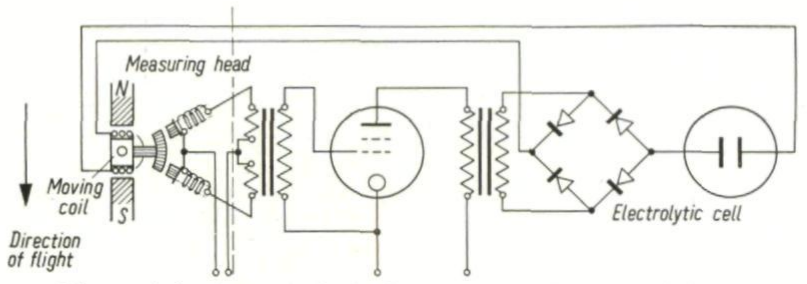
\includegraphics[width=0.8\textwidth]{figs/ctrl-08.png}
  \caption{Scheme of the electronic device for integrating the velocity of the missile.}
  \label{fig:08}
\end{figure}

Two different integrating devices were employed. The first (IG 1) utilized the fact that a gyro under the influence of an acceleration processes at a rate proportional to the acceleration. The angle of precession $B_{iw}$ was proportional to the integral with respect to time of all accelerations, i.e. the value $v_{s}$. The fuel cut-off signal was released when the gyro, reaching the angle of precession $A_{iw}$, closed a properly adjusted contact. The second device (IG 2) determined the velocity by means of a rotating pendulum fettered by an electric current. When the pendulum moved from its zero position under the influence of an acceleration, a bridge became unbalanced (Fig. \ref{fig:08}). Thus a current was caused to flow in the moving coil which fettered the pendulum. The condition of equilibrium was such that the torque caused by the acceleration and the torque of the moving coil compensated each other. The moving-coil current was also proportional to the acceleration. This current was integrated by means of an electrolytic cell especially developed for this purpose The charge $B_{iL}$, of the cell during the flight is proportional to the velocity $v_{s}$. Before launching the cell was charged with $A_{iL}$, in the opposite sense and caused fuel cut-off when the charge $B_{iL}-A_{iL}$ passed through zero.

Because of the required gravity correction, the IG-method is less accurate than the radio method. The latter was to be preferred for another reason. By a minor modification of the base $M$, the influence of errors of the trajectory tangent angle i), on the range $X$ can be eliminated. The equation

\begin{equation}
  X=f(v_{1}, \nu_{1})
\end{equation}

is more accurate than equation (2.1).

If $\nu_{1}$, is slightly different from its assigned value  $\nu_{1}^{*}$, a velocity must be chosen which, in its turn, is also slightly different from its assigned value in order to obtain its correct range. Again we have

\begin{equation}
  X=f(v_{x}, v_{y})\quad\quad(v_{x}=v_{1}\cos{\theta}, v_{y}=v_{1}\sin{\theta}).
\end{equation}

If $v_{x}$ and $v_{y}$ differ only slightly from their assigned values, the following
equations holds:

\begin{equation}
  X=\frac{\partial f}{\partial v_{x}}v_{x}+\frac{\partial f}{\partial v_{y}}v_{y}+E\quad\quad{E=\text{a numerical value}},
\end{equation}

Formula (2.6) can be transformed into

\begin{equation}
  X=\sqrt{\left(\frac{\partial f}{\partial v_{x}}\right)^{2}+\left(\frac{\partial f}{\partial v_{y}}\right)^{2}}=E
\end{equation}

with

\begin{equation}
  \cot{a} = \frac{\partial f/\partial v_{y}}{\partial f/\partial v_{x}}.
\end{equation}

Thus a given range depends only on the rocket velocity in the direction $a$. We eliminate the influence of the angle of the trajectory tangent if we position the base $M$ so that the straight line joining $M$ and the rocket at the time of cut-off contains the angle $a$ (instead of $v_{1}^{*}$) with the vertical. A corresponding correction is not possible with an integrating device fixed to the axis of the rocket. The above partial derivatives were obtained from trajectory calculations.
\end{enumerate}

\subsection{Some Trial Results}

For the average deviation, quoting from memory, we obtained the following
results:

\begin{center}
\begin{tabular}{|l|c|}
  \hline
  Error in line & $z_{50} \pm 4.5$ km \\\hline
  Error in range with cut-off by IG-method & $z_{50} \pm 4.5$ km \\\hline
  Error in range with cut-off by radio & $z_{50} \pm 4$ km \\\hline
\end{tabular}
\end{center}

It should however be said that the last IG-method results were somewhat better than the last radio-method results. The reason for this somewhat surprising result is not known with certainty. We conjectured the following: the range depends also on the position of the rocket at fuel cut-off. If now the thrust (especially after its reduction) is too weak, the rocket travels for a longer time and therefore over a greater distance than originally intended, until it reaches the fuel cut-off velocity. In the case of the radio-method, this causes an error in range only, whereas with the IG-method an error in time is introduced due to the influence of gravity. This error, as can be seen from equation (2.2), operates in the opposite direction. Whether this compensation actually improved the accuracy noticeable is not quite clear.

Part of the observed deviation is naturally caused by the wind and other influences during the time of free flight. The error thus caused was estimated at a few hundred meters.

The influence of the rotation of the earth on the trajectory (some kilometers) made the use of range tables necessary.

\section{The Guide Plane Control of the Special Series}

\subsection{Description}

As already mentioned, the rocket, if controlled by the automatic pilot only, will drift laterally under the influence of lateral forces. On an average this causes a considerable deviation. If, at the instant of fuel cut-off, the rocket has a velocity of say, 1400 m/sec corresponding to an approximate range of 250 km and the lateral wind has an assumed velocity of 20 m/sec, an error in line of about 3.5 km is to be expected. Further noticeable lateral deviations must be expected as a result of the wandering of the course gyro, and asymmetries in thrust. In order to reduce these inaccuracies, some of the V-2 rockets were equipped with guide-plane control. It had been demanded that this control should operate through an additional signal to the automatic pilot. It was intended to operate the rockets with automatic pilot only in the case of interference. Furthermore production problems caused that demand. It may be mentioned here that the radio connection to the V-2 was never jammed.

\begin{figure}[ht]
  \centering
  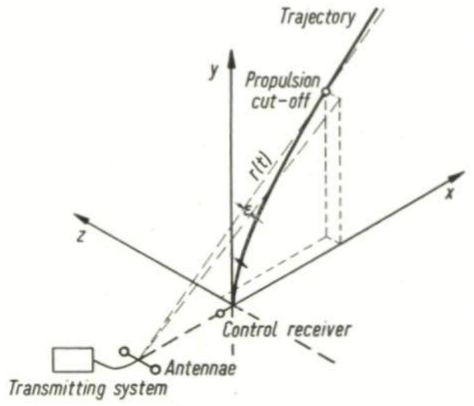
\includegraphics[width=0.6\textwidth]{figs/ctrl-09.png}
  \caption{The radio range control of the V-2.}
  \label{fig:09}
\end{figure}

The guide-plane was produced as follows (Fig. \ref{fig:09}): A transmitter with a Frequency of about 50 mc/sec was positioned at a distance of 10 km behind the launching base, so that transmitter and launching base were contained in the plane intended as guide-plane. The transmitter fed two horizontal dipoles positioned at a distance of about 200 metres from each other. The feeding into the connecting line of the two aerials was effected alternately at two points which had the same distance from the nearer aerial and the distance of about $\lambda/4$ from each other (Fig. \ref{fig:10}). The switching frequency was 50 c/sec and beam characteristics $a$ and $b$ were obtained alternately (the parasitic lobes are suppressed). At the receiver input one obtained a square modulated voltage whose depth of modulation was very approximately proportional to the angle $\varepsilon$ formed by the straight line transmitter—receiver with the guide-plane. An additional modulation of the transmitter of 7 kc/sec made it possible to find out whether the receiver was to the right or to the left of the guide-plane.

\begin{figure}[ht]
  \centering
  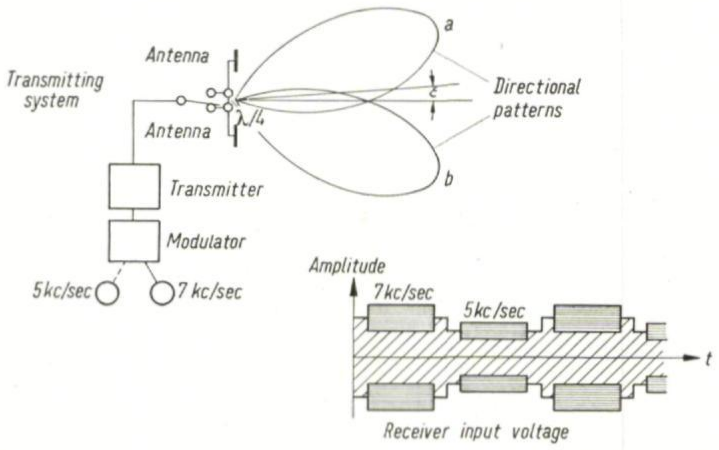
\includegraphics[width=0.7\textwidth]{figs/ctrl-10.png}
  \caption{Transmitting system of the radio control system with directional patterns; in put voltage to the receiver.}
  \label{fig:10}
\end{figure}

The position of the guide-plane was monitored by a control receiver arranged in the desired direction of the guide-plane. At the receiver output in the rocket a voltage was obtained whose positive or negative sign depended on the lateral position (right or left) of the rocket and was proportional to its angular position $\varepsilon$. This voltage was, via a stabilizer network, fed into the amplifier for the control in yaw. This network formed beside the $\varepsilon$ signal also an isodrome control because, in the case of a pure angle control (including its derivatives), the rocket, under the influence of lateral forces or of a gyro deviation, travels at a certain distance parallel to the guide-plane. The isodrome signal destabilized the rocket and therefore had to be chosen sufficiently weak. The guide-plane system was, like all other radio equipments for the V-2, developed for ten frequencies in order to dodge interference.

\subsection[The Control Equations for the V-2 Automatic Pilot and Yaw Control with the Guide-Plane]{The Control Equations for the V-2 Automatic Pilot and\\Yaw Control with the Guide-Plane}

Now we shall consider the problem of finding a suitable form of control equations. The three dimensional motion of a rocket with its six degrees of freedom can be described by six simultaneous differential equations of the second order. The coupling of these equations is considerably reduced if the rocket — like the V-2 — does not roll (this was another reason for aiming at a good stability in roll). It was found that the remaining coupling between pitch and yaw control could be neglected for a rocket with the aerodynamic characteristics and the trajectory of the V-2, so that the motion of the V-2 could be considered separately in each plane.

The stability problem is nearly identical for yaw, pitch and roll. Therefore we shall consider in detail how the equation for control in yaw was obtained, because in this case the additional problem of lateral control by guide-plane had to be dealt with.

\begin{figure}[ht]
  \centering
  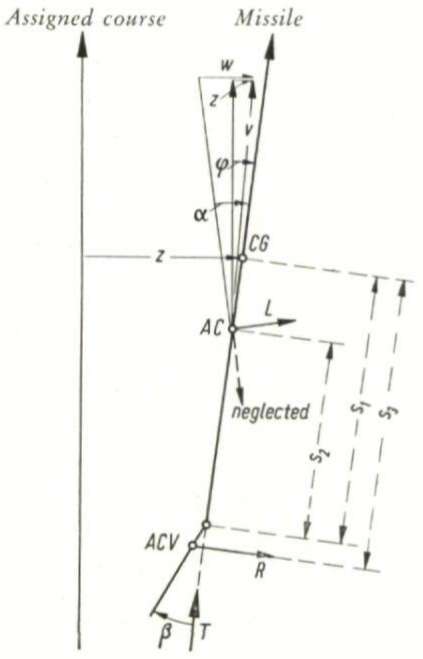
\includegraphics[width=0.4\textwidth]{figs/ctrl-11.png}
  \caption{Diagram of the forces which enter in the yaw control\\CG = Centre fpf gravity, AC = Aerodynamic centre, ADV = Aerodynamic centre of vanes.}
  \label{fig:11}
\end{figure}

Fig. \ref{fig:11} shows the lateral forces. The equation of motion are with good approximation if we take into consideration the little damping forces:

\begin{equation}
  \Theta\frac{d^{2}\varphi}{dt^{2}}+\delta^{*}\frac{d\varphi}{dt}+\frac{L}{a}(s_{1}-s_{2})a=-\frac{\partial R}{\partial\beta}s_{3}\beta,
\end{equation}

\begin{equation}
  m\frac{d^{2}}{dt^{2}}z=\frac{\partial L}{\partial a}a+\frac{\partial R}{\partial\beta}+D^{*}\frac{\varphi}{dt}+T\varphi,
\end{equation}

where

\begin{enumerate}[label={}]
  \item $\Theta=$ moment of inertia,
  \item $L\approx\dfrac{\partial cl}{\partial a}S\dfrac{\rho}{2}v^{2}a=$ lateral force,
  \item $cl=$ lateral force coefficient,
  \item $S=$ cross-section of the rocket,
  \item $\varphi=$ angle between longitudinal axis and assigned course of the rocket,
  \item Functions of functions.

  \item $R=\dfrac{\partial cl_{r}}{a}S\dfrac{\rho}{2}v^{2}\beta$ controller force,
  \item $cl_{r}=$ controller force coefficient,
  \item $\beta=$ controller angle,
  \item $m=$ mass of the rocket,
  \item $T=$ thrust,
  \item $D^{*}\dfrac{d\varphi}{dt}\approx\dfrac{\partial cl}{a}S\dfrac{\rho}{2}v^{2}\dfrac{s^{2}_{1}}{v}\dfrac{d\varphi}{dt}$ damping force,
  \item $\delta^{*}\dfrac{d\varphi}{dt}\approx\dfrac{\partial cl}{a}S\dfrac{\rho}{2}v^{2}\dfrac{s^{2}_{1}}{v}\dfrac{d\varphi}{dt}$ damping moment,
  \item $s_{1}-s_{2}=$ distance between the centre of gravity and the aerodynamic centre,
  \item $s_{3}=$ distance between the centre of gravity and the aerodynamic centre of vanes.
\end{enumerate}

The angle of attack is

\begin{equation}
  a=\dfrac{w-dz/ dt}{v}+\varphi,
\end{equation}

where

\begin{enumerate}[label={}]
  \item w = velocity of lateral wind,
  \item z = lateral distance of the rocket from its assigned trajectory.
\end{enumerate}

If $d/dt$ is written as $p$, from (3.1), (3.2) and (3.3) follows

\begin{equation}
  p^{2}\varphi+\delta p\varphi+c_{1}\varphi-kpz=-kw-c_{2}\beta
\end{equation}

\begin{equation}
  p^{2}z+D p\varphi+C_{1}\varphi-Kpz+C_{2}\beta=-Kw.
\end{equation}

The suitable control equation can be written as follows if we assume that we
are using a passive control network:

\begin{equation}
  \beta(m_{0}+m_{1}p+m_{2}p^{2}+m_{3}p^{3})=\frac{1+a_{10}p+a_{20}p^{2}}{1+T_{1}p+T_{2}p^{2}}a_{0}\varphi+b_{0}\frac{1+b_{10}p}{1+T_{3}p}z+b_{0}\frac{b_{10}}{1+T_{4}/p}\frac{z}{p}.
\end{equation}

The first term on the right hand side signifies the gyro signal, the second the actual guide-beam signal, and the third the additional isodromc control. We still have to express $z$ by the guide beam angle $\varepsilon$:

\begin{equation}
  z=r(t)\varepsilon,
\end{equation}

\begin{equation}
  b_{0}z=e_{0}\varepsilon.
\end{equation}

if we examine the problem of stabilization only.

It can be easily seen that the first term is suitable in the case of gyro control only. Equation (3.5) is to be omitted and equation (3.4) is simplified into

\begin{equation}
  p^{2}\varphi+\delta p\varphi+c_{1}\varphi=c_{2}\beta,
\end{equation}

if we examine the problem of stabilization only.

For a position servo unit a good stabilization is obtained with the equation

\begin{equation}
  m_{0}\beta=a_{0}\varphi(1+a_{10}p)
\end{equation}

and for a velocity servo unit with the equation

\begin{equation}
  m_{1}p\beta=a_{0}\varphi(a_{10}p+a_{20}p^{2}).
\end{equation}

For from (3.9) together with (3.10) and (3.11) respectively we obtain

\begin{equation}
  p^{2}\varphi+p\varphi\left(\delta+\frac{a_{0}a_{10}c_{2}}{m_{0}}\right)+\left(c_{1}+\frac{a_{0}c_{2}}{m_{0}}\right)\varphi=0,
\end{equation}

\begin{equation}
  p^{2}\varphi+p\varphi\left(\delta+\frac{a_{0}a_{20}c_{2}}{m_{1}}\right)+\left(c_{1}+\frac{a_{0}a_{10}c_{2}}{m_{1}}\right)\varphi=0.
\end{equation}

The oscillation about the centre of gravity is additionally damped in the first case by the first, in the second case by the second differential quotient of the control equation. The servo unit was originally rate-coordinated, however, the net hinge-moments of the control vanes actually make $m_{0}$ somewhat different from zero. It is therefore probable that a signal of the form $a_{0}(1+a_{10}p+a_{20}p^{2})$ produces good stability. Naturally, $a_{0}$ would have to be present in the signal even if it effected destabilization, since it determines the assigned course ot the automatic pilot.

The terms in the denominator are unavoidable if a passive control network is used. In the final calculation of an optional transfer function for the signal, they naturally had to be considered; moreover, the coefficient $m_{2}$ carried considerable weight. As mentioned above a network was developed according to equation (3.6), which permitted the control characteristics to be kept constant during the entire control period.

Based on similar considerations, it was at first assumed that the guide-plane signal had also to be formed by a double differentiating network. However, the calculations showed that single differentiation was sufficient. Since, in the case of the guide-plane control, the controlled motion of the rocket is represented by two simultaneous differential equations, the stability calculations become far more extensive than those for the automatic pilot. Moreover, they are less reliable because such calculations can be carried out in practice only for equations with constant coefficients. This is permissible for the automatic pilot because the oscillation about the centre of gravity is sufficiently rapid; however, in the case of the guide-plane control the values thus obtained appear rather questionable because the oscillation of the centre of gravity is very slow. It was found, however, that these calculations give quite a good idea of the stability of the guide-plane control. Control characteristics and transfer functions for the first guide-plane controlled rockets were determined by means of such calculations and produced satisfactory stability.

It was found that during the control period the transfer function could be kept constant, but that the amplification had to be varied. This was accomplished by a cam gear-driven-potentiometer at the input of the yaw control amplifier.

The fact that the end of the propelled part of the trajectory $e_{0}$ had to be varied considerably, unfortunately destroyed to a great extent the effect of the isodromc control, which was also proportional to $e_{0}$. It was not possible to develop methods avoiding this disadvantage.

The denominator term of the guide-plane signal calls for the following remarks: while the denominator terms of the automatic pilot system signal were chosen so small — they were regarded as undesirable — as was technically permissible (attenuation factor of the network) $T_{3}$, was chosen as large as possible in order to filter the signal, but without jeopardizing the stability of the control: the possibility of interference was to be reduced. In the end, filtering was still carried further by a guide-plane signal of the type (approximately)

\begin{equation}
  e_{0}\frac{1=b_{10}p}{(1+T_{3}p)^{2}}z.
\end{equation}

In spite of many efforts we did not succeed in making the lateral control of the rocket really stable during the last seconds before all-burnt. Although the rocket always remained in close proximity to the guide-plane, we often observed an angle between the trajectory tangent at all-burnt and the guide-plane, which could not be neglected. The systems of equations for the control in roll and pitch are somewhat different from those for the control in yaw, but the difference is not material and, therefore, we do not consider them here.

\subsection[The Methods Used for Stability Control. — Numerical Methods and Analogue Computers]{The Methods Used for Stability Control. — Numerical\\Methods and Analogue Computers}

The numerical investigations of the stability problem were almost exclusively carried out by the method of small disturbances, i.e. the roots of the characteristic equation of the system of differential equations were examined. For this purpose, the method of examining the determinant of the highest order did not appear to be particularly suitable; instead, damping regimes were calculated specially, by a method using the conditions for the coefficients. The results ot this method may be explained in a few words: if for instance the other coefficients of the guide-plane control are given, the limits are obtained with which $b_{0}$ and $b_{10}$ may be chosen, if the damping of the oscillation should not be less than a certain value. In principle, the method requires a considerable amount ot calculation; however, approximate methods were developed to reduce the labour.

Investigations into the stability were also carried out with the help of the NYQUIST method, but this was not so popular.

The stability of the pure automatic pilot control was also investigated with the help of an electro-mechanical analogue computer, because it was not possible to consider the backlask of the servo-unit and the non-linearities in the calculation. The computer was a kind of moving-coil voltmeter (Fig. \ref{fig:12}) whose pointer had been enlarged to a pendulum. A small eddy current brake made it possible to adjust the damping of the oscillations of the pendulum. By tilting the pendulum in a plane perpendicular to its axis, its natural frequency could be altered. The following equation was obtained for the free oscillations of the pendulum:

\begin{equation}
  m_{p}^{2}p^{2}\varphi+d_{m}p\varphi+m_{p}gr\cos{\gamma}\cdot{\varphi}=0
\end{equation}

where
\begin{enumerate}[label={}]
  \item $m_{p} =$ mass of the pendulum.
\end{enumerate}

\begin{figure}[ht]
  \centering
  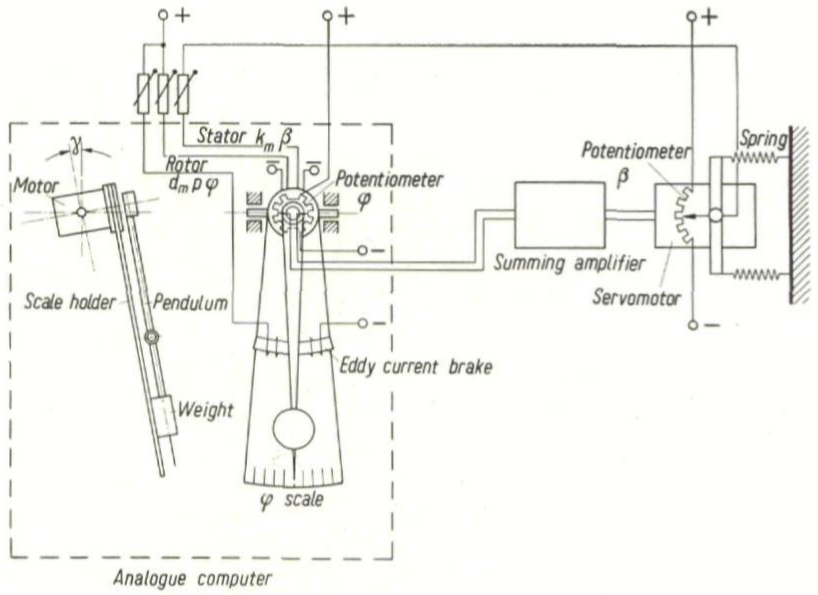
\includegraphics[width=0.7\textwidth]{figs/ctrl-12.png}
  \caption{Autopilot control simulation: block diagram.}
  \label{fig:12}
\end{figure}

The design data were chosen in such a way as to give the pendulum the particular natural frequency and damping characteristic for the rocket in any point of the controlled part of its trajectory.

In order to investigate the stability of the control system a voltage was determined, with the help of a potentiometer, which was proportional to the angle $\varphi$ between the axis of the pendulum and the vertical (the arrangement was such that this angle was identical with the angle $\varphi$ between the axis of the rocket and its assigned course). This voltage was fed into a mixer unit which operated the servo-unit. The servo-unit carried a potentiometer which produced a voltage proportional to the deflection fi of the controller this voltage exercised a proportional torque on the pendulum. The hinge-moment set up at the servo-unit during flight was imitated by a spring coupling. According to the above the equations for the whole system were:

\begin{equation}
  m_{p}^{2}p^{2}\varphi+d_{m}p\varphi+m_{p}gr\cos{\gamma}\cdot{\varphi}+k_{m}\beta=0,
\end{equation}

\begin{equation}
  m_{0}\beta+m_{1}p\beta+m_{2}p^{2}\beta=a_{0}\varphi\frac{1+\hdots}{1+\hdots},
\end{equation}

this being identical with the system of equations for the pure automatic pilot control. It was observed how the system returned to zero after a disturbance.

The imitation of the system of equations for the guide-plane control seemed to be practically impossible in an electro-mechanical analogue computer, especially because the coefficients had to be variable with time. Therefore an electronic analogue computer had to be developed for these stability investigations. This contained essentially a number of integrators and potentiometers operated by cam shafts. It was possible with the help of these potentiometers to reproduce the variation with time of the coefficients of the system of equations.

\begin{figure}[ht]
  \centering
  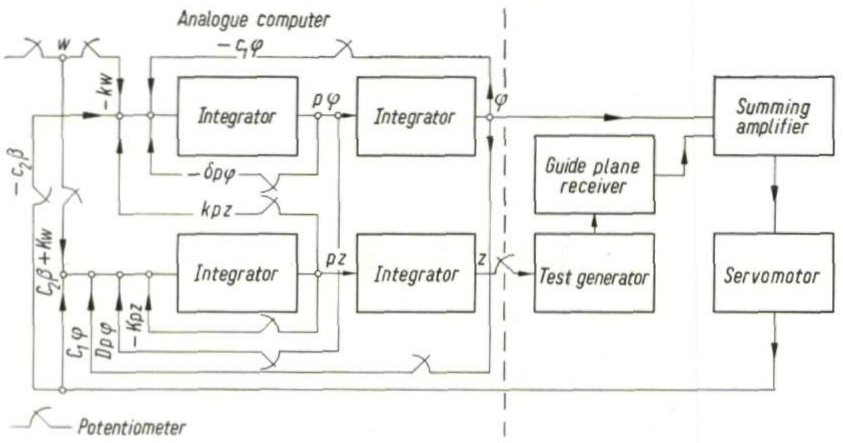
\includegraphics[width=0.75\textwidth]{figs/ctrl-13.png}
  \caption{Radio control simulation: block diagram.}
  \label{fig:13}
\end{figure}

Fig. \ref{fig:13} shows the basic diagram of the computer. One recognizes at once that the input voltage of the two integrators on the left is p-z and p-if, if one approaches the input via the integrator; by adding the voltage fed into the inputs we sec that yields:

\begin{equation}
  p^{2}\varphi=-\delta p\varphi-c_{1}\varphi+kpz-kw-c_{2}\beta,
\end{equation}

\begin{equation}
  p^{2}z=Dp\varphi+C_{1}\varphi-Kpz+Kw+C_{2}\beta.
\end{equation}

The analogue computer thus imitates the equations of the motion of the rocket. The control equation (3.6) is represented by the control elements themselves.

It should be mentioned that the servo-unit was loaded by a leaf spring whose point of support was varied with time in such a way as to imitate the hinge-moment correctly at any time.

Between the output of the analogue computer and the input of the guide-plane receiver which, according to section 3.1, supplies at its output the sum of the actual guide-beam signal and of the isodrome signal was installed a specially developed control generator. By the voltage $\varepsilon=z/r(t)$ this generator was modulated so that at its output it delivered a voltage curve corresponding to the one occurring at the input of a receiver placed at the angular distance $\varepsilon$ from the guide-plane (see Fig. \ref{fig:10}).

\begin{figure}[ht]
  \centering
  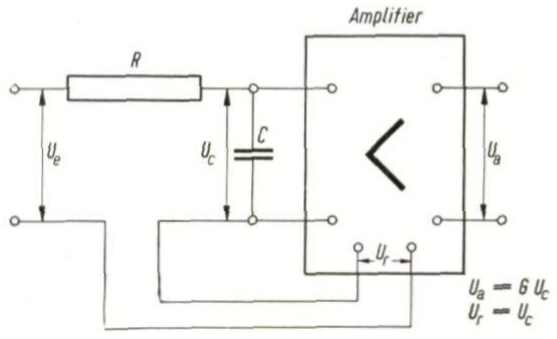
\includegraphics[width=0.55\textwidth]{figs/ctrl-14.png}
  \caption{Principle of an integrating amplifier.}
  \label{fig:14}
\end{figure}

The integrators consisted of capacitors which were charged via resistances. Fig. \ref{fig:14} shows the principle. The condenser voltage is fed-back into the input circuit via a buffer amplifier. Thus we have

\begin{equation}
  U_{a}=\frac{1}{pC}\frac{U_{e}}{R}G
\end{equation}

as long as one operates on the linear part of the amplifier characteristic. If the amplification of the feed-back-loop is somewhat different from 1 the integration is no longer ideal; however, it was possible without great difficulty to keep the time constant greater than ten minutes for half an hour if the resistance $R$ was not too small.

In order to avoid the difficulties which usually occur with a number of D.C. amplifiers in series, the inputs and outputs of the integrators carried 500 c/sec voltages. The input voltages were summed up, the total voltage rectified with a phase-sensitive detector, then the integration carried out and finally the integrated value used to modulate at 500 c/sec suppressed carrier system (see Fig. \ref{fig:15}). The feeding back as described above was carried out with 500 c/sec from output to input of the integrator.

\begin{figure}[ht]
  \centering
  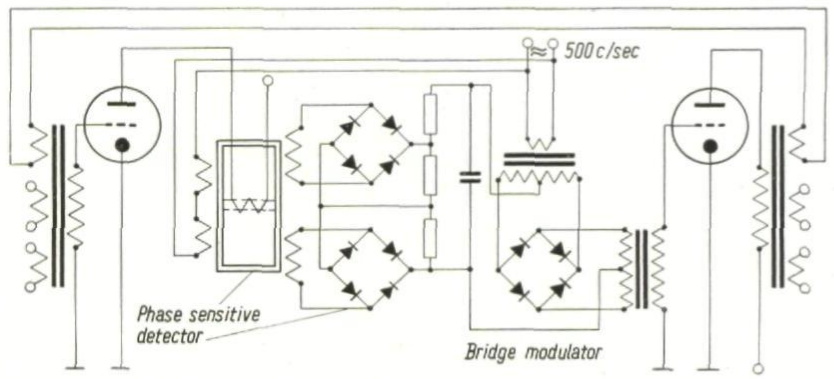
\includegraphics[width=0.75\textwidth]{figs/ctrl-15.png}
  \caption{Simplified circuit of an integrating amplifier.}
  \label{fig:15}
\end{figure}

The operation of the computer was made rather difficult by the necessity of changing a cam shaft if the time function of the coefficient was to be altered. It was therefore intended to equip the potentiometers with step-by-step selectors and to operate these with the help of perforated tape.

The investigations carried out with the electronic analogue computer were of great importance, especially for the solution of the problem of finding the optimum control characteristic and the optimum transfer function for the guide-plane control,

\subsection{Trial results}

The probable error of the rockets with guide-plane control was within one or two kilometres. This error was caused mainly by the angle between the direction of the trajectory tangent at all-burnt and the guide-plane (deviation of 0.1$^{\circ}$ causes in the case of a range of 250 km a lateral deviation of about 400 m). We were convinced that the probable error would be considerably below one km if the problem of improving the damping of the control immediately before all-burnt could be solved.

\section{High Precision Control without Radio}

\subsection{Description}

The integration units had been developed for a V-2-control without radio. But a combination of the described control system with a fuel cut-off unit containing an integrator fixed to the rocket axis could not be expected to produce good accuracy, for the following reasons:

\begin{enumerate}
  \item The gyros precessed too much under the influence of the considerable accelerations.

  \item The integration of the axial acceleration, and the use of the integrated value for the cut-off signal is, as wc have seen, not very advantageous. — More- over, wc had no idea how to supplement this control system by an additional lateral guidance.
\end{enumerate}

In order to remedy this, the following control system without radio was developed: A stabilized platform in Cardan suspension was built into the rocket. By means of three gyros this platform did not alter its direction in space. The angles between the three rocket axes and the platform were used as control quantities for the automatic pilot. Such a platform has a much better stability than a single gyro.

The pick-up of the integrator was mounted on this platform in such a way as to measure the component of the rocket acceleration in the direction a, which was used as measuring direction for the measurement of the rocket velocity by radio. Thus the determination of the fuel cut-off time by means of the integrator becomes theoretically equivalent to its determination by means of radio measurement. Only objection: the term for the correction of gravity which takes the form of

\begin{equation}
  v_{g}=g\cos{a}\cdot{t_{1}^{*}}
\end{equation}

is exact only if the time $t_{1}$, up to all-burnt docs not differ from its value $t_{1}^{*}$ used
in the calculation.

For additional lateral guidance — substitute for guide-plane control — a so-called lateral integrator was developed. An acceleration pick-up was mounted on the stabilized platform in such a way as to measure the acceleration perpendicular to the plane of the trajectory. The pick-up produced a current proportional to this acceleration. A network which in principle performed a double integration of this current yielded the expression

\begin{equation}
  b_{0}z(1+b_{10}p)
\end{equation}

which was used for the control instead of the guide-plane signal. It was not intended to use an integral signal for the time being. The probable error of the firings without additional guidance (only a limited number was available) amounted to

\begin{equation*}
  \begin{split}
    x M&=\pm3.4\text{ km},\\
    250&=\pm2.7\text{ km}.
  \end{split}
\end{equation*}

These rockets were equipped with the electronic integrator. The additional lateral guidance by means of the lateral integrator could only be tried once. The result was a lateral deviation of 0.5 km.

\subsection{Principle of Stabilized Platform and Lateral Integrator}

Fig. \ref{fig:16} is a basic diagram of the stabilized platform. Each of the three gyros has one degree of freedom. If, due to a rotation of the Cardan suspension, a friction torque becomes effective, the respective gyro begins to precess and exerts on the platform a torque of equal magnitude in the opposite direction.

\begin{figure}
  \centering
  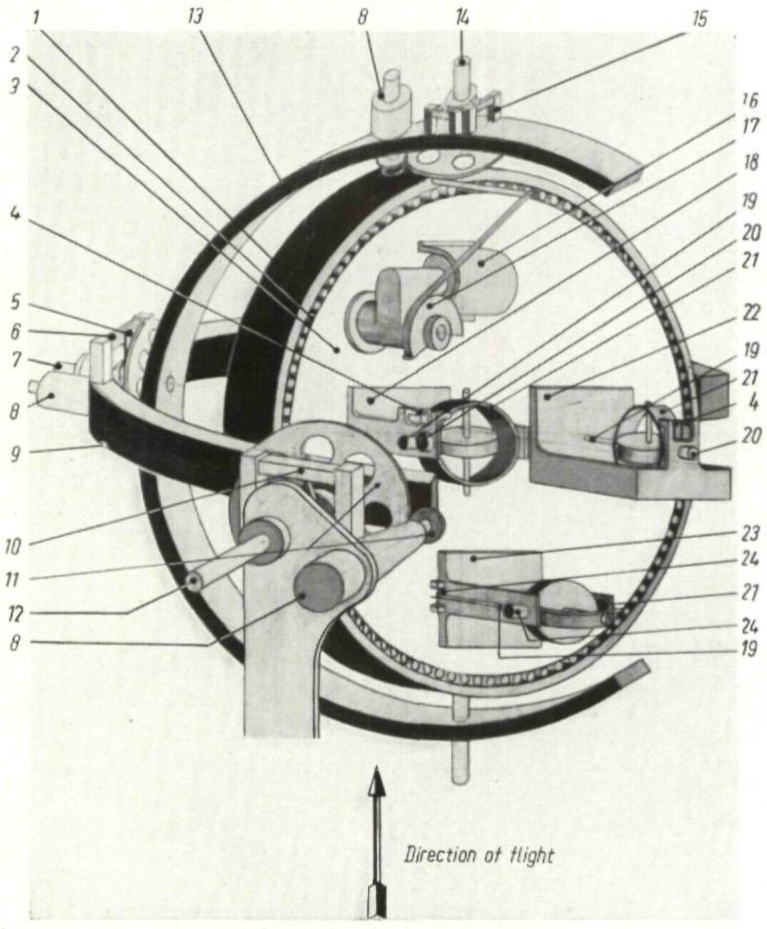
\includegraphics[width=0.7\textwidth]{figs/ctrl-16.png}
  \caption{
    Sketch of the stabilized platform.\\[0.5em]
    \begin{minipage}{0.95\linewidth}
      \centering
      \begin{tabular}{>{\raggedright\arraybackslash}p{0.3\linewidth}
                      >{\raggedright\arraybackslash}p{0.3\linewidth}
                      >{\raggedright\arraybackslash}p{0.3\linewidth}}
        1: Bearing ring & 2: Wire ball bearing & 3: Stable platform \\
        4: Contact of precession & 5: Slider & 6: Yaw pick-off \\
        7: Yaw axis & 8: Torque motor & 9: Outer gimble \\
        10: Pitch pick-off & 11: Gear train & 12: Pitch axis \\
        13: Inner gimble & 14: Roll axis & 15: Roll pick-off \\
        16: Program motor & 17: Curved disc & 18: Pitch gyroscope \\
        19: Precession axis & 20: Torque magnet & 21: Gimble \\
        22: Yaw gyroscope & 23: Roll gyroscope & 24: Magnet \\
      \end{tabular}
    \end{minipage}
  }
  \label{fig:16}
\end{figure}

The platform retains its direction in space. If the gyro has precessed through a certain angle it closes a contact supplying current to the respective supporting motor. This motor then exerts a torque on the platform greater than the possible friction torque. The gyro begins to vibrate around its precession axis. The platform too vibrates somewhat, but the amplitude of its vibration is negligibly small. For good stability of the platform it is essential that the gyros have very little friction about their precession axis.

The change of direction in pitch was carried out as follows: a motor rotated the platform relative to the outer casing of its needle bearings. Naturally, the Cardan suspension ring rotates and not the platform. The potentiometer $D$ supplies a voltage to the servo-units and the rocket changes its direction until the original constellation of longitudinal axis of the rocket and the Cardan suspension ring has been restored.

The simple co-ordination of gyro and supporting motor on which our description is based, no longer holds in the case of the changes in direction, but this is not a fundamental difficulty.

\begin{figure}[ht]
  \centering
  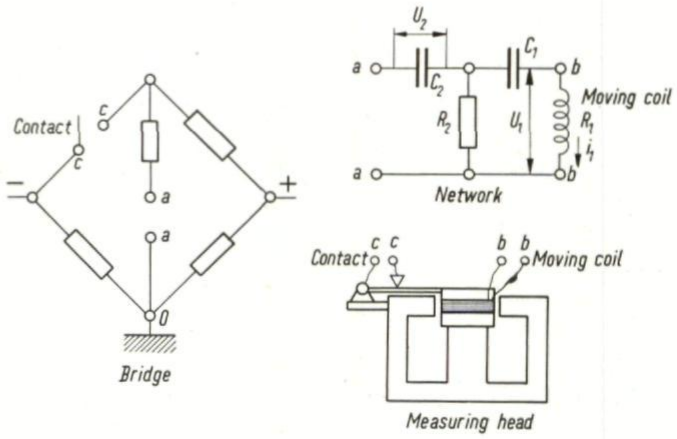
\includegraphics[width=0.6\textwidth]{figs/ctrl-17.png}
  \caption{The device for integrating the acceleration in yaw: sketch of the measuring head; principle of the bridge network.}
  \label{fig:17}
\end{figure}

Fig. \ref{fig:17} shows the lateral integrator. A moving coil which dips into a magnet - the system was similar to a permanent dynamic loudspeaker — was built into the zero branch line of an emergency bridge circuit. Between the opposite points of the bridge and the moving coil is a network. One of the branches of the bridge is replaced by a switch which opens if the depth of the moving coil in the magnet exceeds a certain value. If the apparatus is switched on the coil vibrates with a relatively high frequency about the position thus determined. The mean value of the current in the coil is proportional to the acceleration exerted on the coil in the direction of its axis. Its polarity changes with the direction of the acceleration $i_{1}\sim d^{2}z/dt^{2}$.

The voltage at the terminals a a of the network is

\begin{equation}
  U_{2}=\frac{1}{C_{1}C_{2}R_{2}}\int\int i_{1}dt\cdot dt+C_{1}(R_{1}+R_{2})\int i_{1}dt
\end{equation}

or

\begin{equation}
  U_{2}=kz\left[1+p(C_{1}R_{1}+C_{1}R_{2})\right]  .
\end{equation}

The voltage $U_{2}$, thus contains a component proportional to $z$ and another proportional to $dz/dt$. A signal was obtained similar to the one supplied by the guide-plane receiver, feeding $U_{2}$ into an amplifier whose gain was varied by means of a cam shaft driven potentiometer. The output voltage of the amplifier was fed into the mixer unit.

A moving coil system pick-up would have given too large a systematic error. A component of the longitudinal acceleration proportional to the angle of deflection would have been included in the measurement. If a system had been chosen which avoided the vibration of the moving coil, friction would have been intolerable.

\section[Special Equipment for the Control of the V-2 which was in Course of Development]{Special Equipment for the Control of the V-2 which\\was in Course of Development}

\subsection{The Guide-Line Control}

To protect the radio yaw control better against interference and also in order to make a radio pitch control possible, i. e. a control in two planes vertical to each other, a guide-line system in the 50 cm band was developed.

A continuous wave-transmitter fed the antenna equipment of a radar set, i. e.
a dipole rotating eccentrically within a parabolic reflector. The airborne
receiver determined the angular distance between the pilot beam and the radius
vector to the rocket as an altitude component $\varepsilon_{h}$ and a lateral component $\varepsilon_{v}$. It was similar in operation to the receiver of the radar sets. Due to the horizontal polarization of its aerial, the output voltage of the receiver — making certain approximations — was

\begin{equation}
  U_{3}=k_{1}(2\varepsilon_{v}\sin{\omega t}+\varepsilon\cos{\omega t})+k_{\text{II}}\cos{2\omega t},
\end{equation}

where $\omega=$ frequency of rotation of dipole. The term $k_{\text{I}}$ is led to two phase- sensitive rectifier circuits, into which are fed additional voltages $k_{\text{III}}\cos{\omega t}$ and  $k_{\text{III}}\sin{\omega t}$ respectively. At the output the circuits supplied directional voltages proportional to $\varepsilon_{h}$ and $\varepsilon_{v}$ in amplitude. The voltages $k_{\text{III}}\cos{\omega t}$ and $k_{\text{III}}\sin{\omega t}$ were obtained from $k_{\text{II}}\cos{2\omega t}$  by frequency division. Since no experience was available as to how a guide-plane control device would behave when the guide-plane was being turned, the first lay-out of this set was planned so that the yaw control signal would control the rocket laterally, whereas the pitch control signal was transferred to the ground and this made the reflector follow the rocket vertically. This set was under trial, but has not yet been used for the actual control of a rocket. We were anxious to know whether the mechanical accuracy of the large 7 m parabolic mirror would be sufficient for following the change of direction without trouble.

A radio pitch control would have had the important advantage that the location of the stationary equipment on the ground would have become uncritical for the radio measurement of the velocity.

\subsection[Additional Apparatus for Improving the Accuracy of the All-Burnt Signal]{Additional Apparatus for Improving the Accuracy of the\\All-Burnt Signal}

The range of the V-2 depended, apart from the all-burnt velocity and its direction, primarily upon the co-ordinates of the all-burnt spot $x_{1}$ and $y_{1}$ which normally deviate somewhat from their assigned values. For a better approximation we may replace equation (2.6) by the following relation:

\begin{equation}
  X=x_{1}+\frac{\partial f}{\partial y_{1}}+\frac{\partial f}{\partial v_{x}}\partial v_{x}+E_{2}
\end{equation}

($E_{2}=$ a numerical value). Transforming this equation as was done with equation (2.4), we get

\begin{equation}
  X=k_{1}v_{a}+k_{2}r_{\delta}+E_{2},
\end{equation}

\begin{equation}
  k_{2}=\sqrt{1+(\partial f/\partial y)^{2}},
\end{equation}

\begin{equation}
  \cot{\delta}=\partial  f/ \partial y.
\end{equation}

Thus it is sufficient to measure the component $r_{\delta}$ of the distance covered by the rocket in a direction inclined at an angle $\delta$ with the vertical, and at an angle $\Theta$) with the relevant plane of yaw control, and to consider this component as the so-called ``way-correction", when determining the all-burnt point. The electronic ``longitudinal integration method" makes it possible to determine $r_{\delta}$ in a simple manner: a second pick-up, which measures the acceleration in the direction $\delta$, is placed on the stabilized platform, and the resulting current is integrated twice.

The radio measurement supplied the way-correction with satisfactory accuracy provided a second receiver unit was placed not too far away from the launching base. Labour developments were under way to incorporate the way-correction $k_{2}r_{\delta}$, in both cut-off procedures.

With the radio cut-off procedure the way-correction factor was used to alter the frequency of the WIEN bridge. With the integrator cut-off procedure it was intended to unload additionally, by a current proportional to the twice integrated measurement current, the electrolytic cell, which caused fuel cut-off when the charge passed through zero.

The additional equipment necessitated by the introduction of the way-correction was rather bulky. Devices were developed, therefore, which introduced, instead of a way-correction, a time-correction into the switching-off circuits.

The deviation of the distance all-burnt point-launching base from its calculated value was approximately proportional to the difference between the time required for the flight and its assigned value $t_{1}-t_{1}^{*}$.

Instead of (5.3) we can, therefore, write approximately

\begin{equation}
  X\approx k_{1}v_{a}+k_{3}(t_{1}-t_{1}^{*})+E_{3}.
\end{equation}

With regard to the radio cut-off procedure, the frequency of the WIEN bridge was changed by a synchron-motor which began to rotate at the moment of launching. The first firing tests with this arrangement yielded satisfactory results.

With regard to the integration procedures, it was intended to change the position of the switching contact (IG 1) by a synchron-motor so as to send a constant additional current through the electrolytic cell (IG 2). These developments were not very far advanced, although a time-correction would have considerably reduced the apparent velocity compensation error which is also proportional to $t_{1}-t_{1}^{*}$.

\end{document}
